\documentclass{article}

% Language setting
% Replace `english' with e.g. `spanish' to change the document language
\usepackage[spanish]{babel}

% Set page size and margins
% Replace `letterpaper' with `a4paper' for UK/EU standard size
\usepackage[letterpaper,top=2cm,bottom=2cm,left=3cm,right=3cm,marginparwidth=1.75cm]{geometry}

% Useful packages
\usepackage{amsmath}
\usepackage{graphicx}
\usepackage[colorlinks=true, allcolors=blue]{hyperref}

\usepackage{float}


%%%%%%%%%% Start TeXmacs macros
\newcommand{\tmop}[1]{\ensuremath{\operatorname{#1}}}
%%%%%%%%%% End TeXmacs macros


\providecommand{\keywords}[1]
{
  \small	
  \textbf{\textit{Keywords---}} #1
}

\title{PRUEBAS CON LA MEMORIA CACHÉ
Computación Paralela y Distribuida}
\author{Angel Andres Bejar Merma\\
  \small Universidad Nacional de San Agustin\\
  \small abejar@unsa.com\\
  \small Ciudad de Arequipa
  %\date{\today} 
}


\begin{document}

    \maketitle



%% Aquí podemos añadir un resumen del trabajo (o del artículo en su caso) 
  \begin{abstract}
    El alumno debe realizar un informe en formato artículo (en Latex) donde la implementación, resultados y análisis de la ejecución para los siguientes problemas:
  \end{abstract}
    
  \keywords{Computacion Paralela,Memoria Cache,Valgrind, Matrices }
%\begin{abstract}



%\end{abstract}

%\vspace{5mm} %espacio vertical usar en imagen

\section{Practica 2}

\begin{enumerate}
  \item \textbf{Implementar en C/C++ la multiplicación de matrices clásica, la versión de tres
  bucles anidados y evaluar su desempeño considerando diferentes tamaños de matriz.}

  Las matrices cuadradas  N*N \cite{cormen2022introduction}se definen   con una complejidad de O(n$^2$ ), por lo que, la complejidad de multiplicación matrices cuadráticas es de O(n$^3$ )
Como se puede ver en la fig \ref{fig:figura2} mientras mas grande sea la matriz ,mas lento sera el tiempo de ejecución, esto se debe a que una de las matrices se se lee como el primer algoritmo
el cual necesita desalojar la memoria de las lineas anteriores y hacer este proceso toma mas
tiempo. ya que generara n*n fallos para la segunda matriz y este proceso de alojar y desalojar
la memoria demora en tiempo de ejecución.





\begin{figure}[h!]
    \centering
   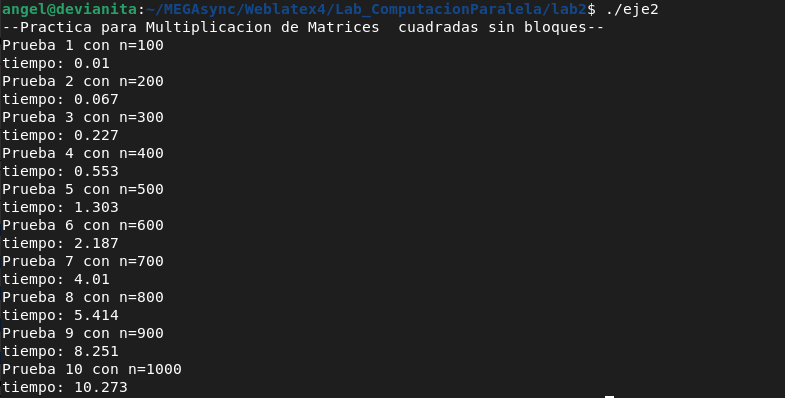
\includegraphics[width=1\linewidth]{imagenes/Captura de pantalla de 2023-09-24 19-40-19.png}
   \caption{Muestras los tiempos de ejecución para matrices cuadráticas}
   \label{fig:figura2}
\end{figure}


  \item \textbf{Implementar la versión por bloques (investigar en internet), seis bucles anidados, evaluar su desempeño y compararlo con la multiplicación de matrices clásica.}
  
\subitem \textbf{La matriz por bloques:} 
una matriz por bloques o una matriz particionada es una matriz interpretada, caracterizada por estar dividida en secciones llamadas bloques o submatrices. Una matriz por bloques se puede visualizar como la matriz original con una colección de líneas horizontales y verticales que la dividen, o particionan, en una colección de matrices más pequeñas.
  Esta técnica se utiliza para reducir los cálculos con matrices; en expansiones de filas y columnas; y en diversas aplicaciones en \textbf{ciencias de la computación}, incluido el diseño de chips integrados. Un ejemplo es el algoritmo de Strassen para la multiplicación de matrices rápida, así como la codificación Hamming(7,4) para detección de errores y recuperación de datos en las transmisiones digitales\url{https://es.wikipedia.org/wiki/Matriz_por_bloques}.

  \begin{figure}[h]
    \centering
   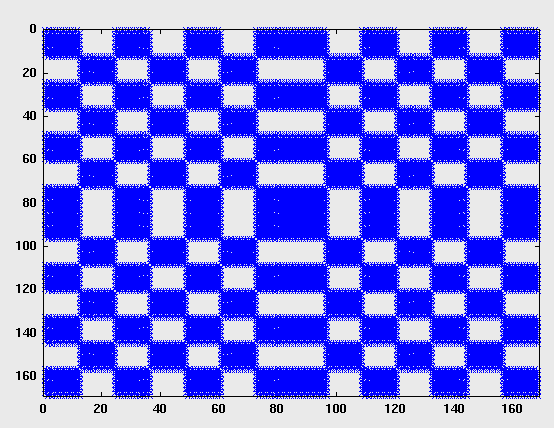
\includegraphics[width=0.5\linewidth]{imagenes/BlockMatrix168square.png}
   \caption{Una matriz por bloques de 168×168 elementos con submatrices de 12x12, 12x24, 24x12 y 24x24. Los elementos distintos de cero están en azul, los elementos cero están en gris}
 
\end{figure}

  

  Las pruebas se realizaron en  bloques de tamaño 10, 50, 100 y matrices cuadradas de 100, 200, 300, ..., 2000,
  esto se puede ver en las figuras \ref{fig:figura3} \ref{fig:figura4} \ref{fig:figura5}  en los cuales se puede observar que sus tiempo de ejecución es mucho mas corto que una multiplicación de matrices normales. Es se debe a que se define
  el tamaño de bloques, el cual sera cargado en cache, y nos permite hacer que las variables locales
  se almacenen en registros de tal modo que no se requiere lectura\slash escritura para acceder a esta
  variable, que la matriz siempre sera guardada en la RAM y que el bloque siempre se alojara en
  la cache.Ademas se ve en detalle la comparación \ref{fig:compara} .



  \begin{figure}[h!]
    \centering
   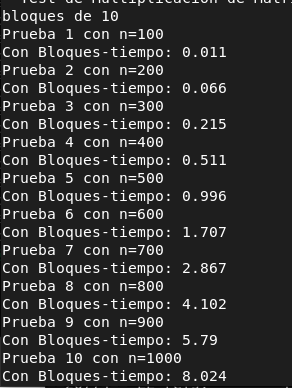
\includegraphics[width=0.5\linewidth]{imagenes/Captura de pantalla de 2023-09-24 21-06-50.png}
   \caption{Tiempos de ejecución para bloques de 10}
   \label{fig:figura3}
\end{figure}

\begin{figure}[h!]
    \centering
   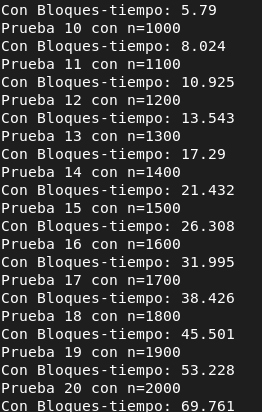
\includegraphics[width=0.5\linewidth]{imagenes/Captura de pantalla de 2023-09-24 21-06-35.png}
   \caption{Tiempos de ejecución para bloques de 10}
   \label{fig:figura3}
\end{figure}




\begin{figure}[h!]
    \centering
   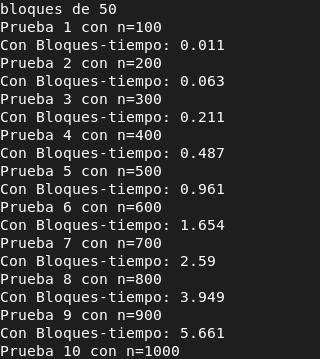
\includegraphics[width=0.5\linewidth]{imagenes/Captura de pantalla de 2023-09-24 20-51-51.png}
   \caption{Tiempos de ejecución para bloques de 50}
   \label{fig:figura4}
\end{figure}

\begin{figure}[h!]
    \centering
   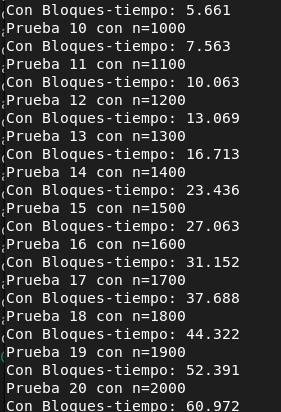
\includegraphics[width=0.5\linewidth]{imagenes/Captura de pantalla de 2023-09-24 20-52-17.png}
   \caption{Tiempos de ejecución para bloques de 50}
   \label{fig:figura4}
\end{figure}



\begin{figure}[h!]
    \centering
   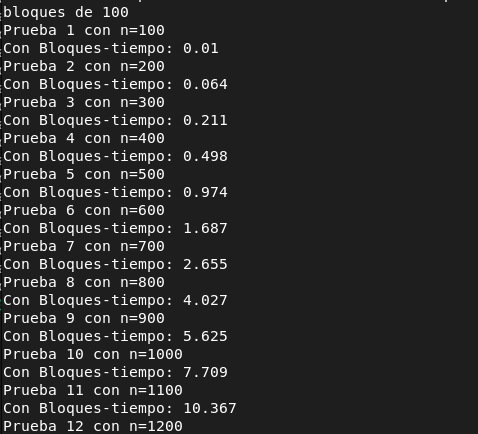
\includegraphics[width=0.5\linewidth]{imagenes/Captura de pantalla de 2023-09-24 20-48-57.png}
   \caption{Tiempos de ejecución para bloques de 100}
   \label{fig:figura5}
\end{figure}


\begin{figure}[h!]
    \centering
   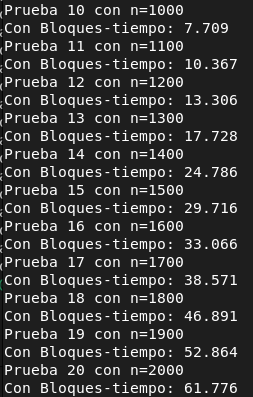
\includegraphics[width=0.5\linewidth]{imagenes/Captura de pantalla de 2023-09-24 20-49-23.png}
   \caption{Tiempos de ejecución para bloques de 100}
   \label{fig:figura5}
\end{figure}

\begin{figure}[h!]
    \centering
   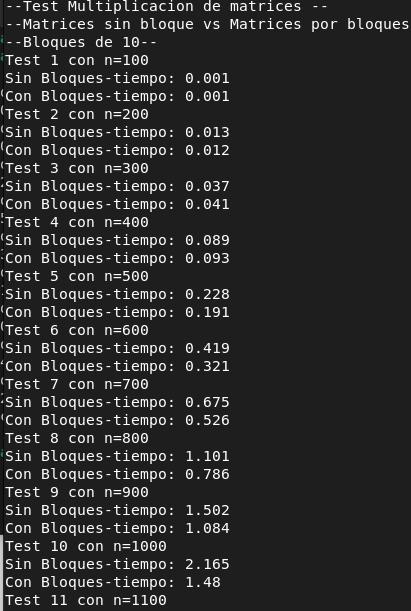
\includegraphics[width=0.5\linewidth]{imagenes/Captura de pantalla de 2023-09-24 20-05-13.png}
   \caption{muestra la comparación de los tiempos de ejecución de la multiplicación de matrices}
   \label{fig:compara}
\end{figure}

\begin{figure}[h!]
    \centering
   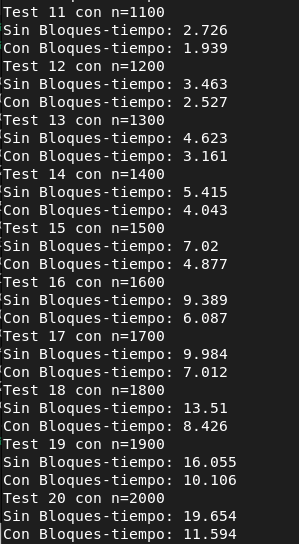
\includegraphics[width=0.5\linewidth]{imagenes/Captura de pantalla de 2023-09-24 20-05-34.png}
   \caption{muestra la comparación de los tiempos de ejecución de la multiplicación de matrices}
   \label{fig:compara}
\end{figure}



  \item \textbf{Ejecutar ambos algoritmos paso a paso, y analizar el movimiento de datos entre la memoria principal y la memoria cache. Hacer una evaluación de acuerdo a la complejidad algorítmica.}
\\
\\
  Matriz A y B N*N con N = 6:\newline
  
\textbf{Para Multiplicación de Matrices normal}

 Primero se lee A[0][:] y luego B[:][0]  lo cual nos dice que  A[0][:] tendra  una falla de cache a la hora de leer este dato, mientras
que para B[:][0] cometerá N fallas de cache ya que tendrá que desalojar las filas anteriores
para alojar una nueva fila, esto generara demoras en tiempo de ejecución. y mientras el
nivel de cache sea mayor, esta sera mas lenta.

Este Proceso ocurre N veces A y para B N*N veces lo cual la localidad de los datos en B
es temporal.

\textbf{Para Multiplicación de Matrices por bloques}


El tamaño del bloque se define de manera que solo este bloque se carge en la memoria caché, es decir, de la 
matriz A y la matriz B solo se carga una parte de bloque ,cada uno de tamaño bsize $\ast$ bsize,
y esto sera multiplicado como un escalar evitando la lectura y escritura para acceder a este
bloque.

Aquí la matriz siempre ira a la RAM mientras que el bloque a la caché, el cual es suficiente
para almacenar los bloques, es decir, $\mid$cache$\mid$ = bsize$^{2}$ + 2 $\ast$ bsize.

Por tanto, las referencias a la matriz A tienen una buena ubicación espacial, ya que se accede
a cada segmento con un paso de 1. Además, también tienen una buena ubicación temporal
ya que todo el segmento está referenciado bsize veces en sucesión. Las referencias a la matriz
B, a su vez, tienen una buena localidad temporal porque se accede al bloque de tamaño
bsize x bsize n veces sucesivamente.
\textbf{Complejidad:}\newline
Tanto la asignación como la liberación de cada matriz ocurre en O(n$^2$ ).

\textbf{Multiplicación de Matrices sin Bloques: } La multiplicación de las matrices A y B se realiza en
O(n$^3$ ).\newline
\textbf{Multiplicación de Matrices por Bloques :} Para la multiplicación, hay dos bucles externos que
varían los bloques dentro de B de tamaño bsize x bsize. Luego, un bucle i que itera sobre las N
filas de A y C, un bucle j para cada columna del bloque B (es decir, bsize veces) y un bucle k
para cada elemento del segmento de A y la línea B (bsize veces).

\[ \frac{N}{\tmop{bsize}} \ast \frac{N}{\tmop{bsize}} \ast N \ast \tmop{bsize}
   \ast \tmop{bsize} = N^3  \]


\


  \item   \textbf{Ejecutar ambos algoritmos utilizando las herramientas valgrind y kcachegrind para obtener una evaluación mas precisa de su desempeño en términos de cache misses.}
  


  \begin{figure}[H]
    \centering
   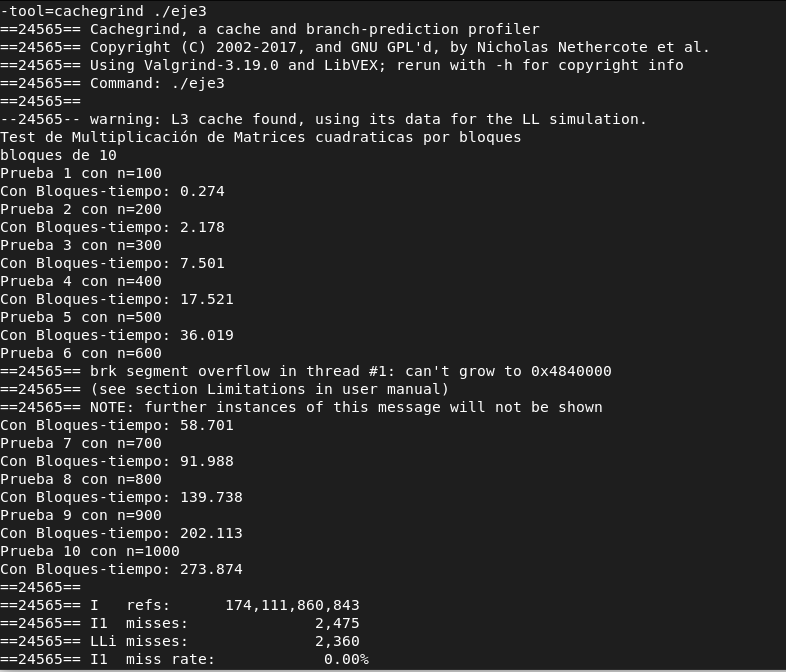
\includegraphics[width=0.8\linewidth]{imagenes/Captura de pantalla de 2023-09-24 22-04-01.png}
   \caption{Evaluación en términos de cache misses  bloque usando kcachegrind}
\end{figure}

\begin{figure}[H]
    \centering
   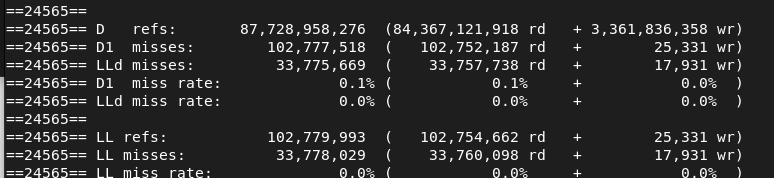
\includegraphics[width=0.8\linewidth]{imagenes/Captura de pantalla de 2023-09-24 22-04-39.png}
   \caption{Evaluación en términos de cache misses bloque  usando kcachegrind}
\end{figure}


\begin{figure}[H]
    \centering
   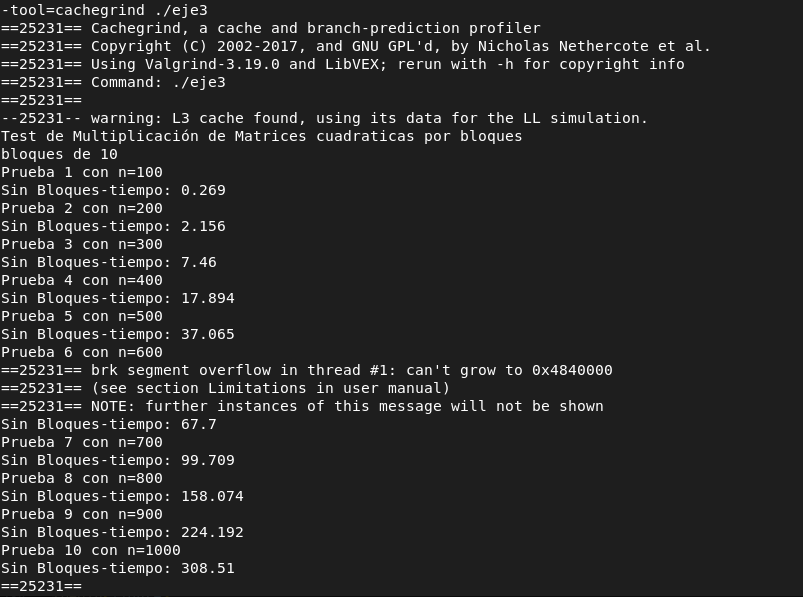
\includegraphics[width=0.8\linewidth]{imagenes/Captura de pantalla de 2023-09-24 22-36-24.png}
   \caption{Evaluación en términos de cache misses sin bloque kcachegrind }
\end{figure}

\begin{figure}[H]
    \centering
   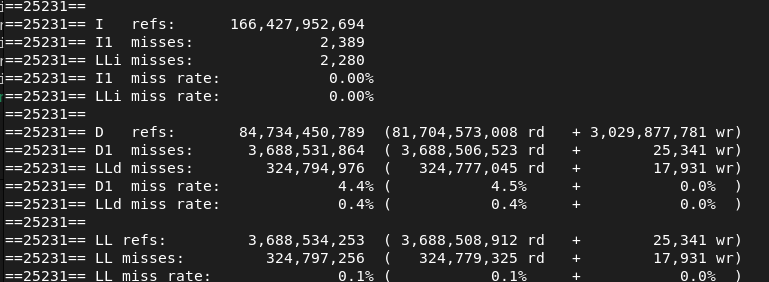
\includegraphics[width=0.8\linewidth]{imagenes/Captura de pantalla de 2023-09-24 22-36-46.png}
   \caption{Evaluación en términos de cache misses sin bloque kcachegrind}
\end{figure}








\end{enumerate}




\begin{figure}
    \centering
   %\includegraphics[width=0.25\linewidth]{frog.jpg}
   %\caption{\label{fig:frog}This frog was uploaded via the file-tree menu.}
\end{figure}




\newpage








	
\section{Conclusión}

El algoritmo está implementado en C++ y alojado en el siguiente  \url{https://github.com/ubuangel/Weblatex4/tree/main/Lab_ComputacionParalela}
Existen muchas formas de implementar la multiplicación de matrices segun la forma de acceder a 
 la memoria, por lo cual cada uno tiene sus propias especificaciones. En esta practica se
hizo la multiplicación por bloques y la forma clásica , de lo cual podemos decir que la multiplicaciones por
bloques nos ayuda a disminuir la tasa de perdida de cache haciendo mejoras en la localidad espacial
y temporal del acceso a la memoria \cite{pacheco2011introduction}

\vspace{20 mm}






    \bibliographystyle{apalike}
    \bibliography{referencias}

\end{document}